\documentclass[10pt]{article}
\usepackage[margin=0.65in]{geometry}
\usepackage{amsmath}
\usepackage{booktabs,tabularx,array,graphicx,xcolor,enumitem,float}
\usepackage{hyperref}
\usepackage{pgfplots}
\pgfplotsset{compat=1.18}
\hypersetup{colorlinks=true,urlcolor=blue,linkcolor=blue}
\setlength{\parindent}{0pt}
\setlength{\parskip}{3pt}
\setlist{nosep,leftmargin=*}
\renewcommand{\arraystretch}{1.08}

\begin{document}\small
\begin{center}
{\Large\bfseries 602 Offline LSTM Gate vs. Offline AMPM}\\[2pt]
{\small Matched-input capacity sweep for \texttt{602.gcc\_s-734B} --- seed 7}
\end{center}

\section*{Experiment contract}
\begin{center}\scriptsize
\begin{tabularx}{\textwidth}{@{}lX@{}}
\toprule
Status & \textbf{PASS}; all five capacities passed canonical decompressed-content SHA256 checks.\\
Primary comparison & \texttt{offline\_ampm} vs. \texttt{offline\_lstm\_h<width>}; identical keyed ListReplayer transport.\\
Shared information & Current cache-line address, causal prior address history, and equivalent causal 64-page bitmap/LRU state. PC is replay identity only.\\
Forbidden information & Hit/miss, cycle, queues, metadata, and future evaluation rows.\\
Data split & 0--20M train, 20--25M guard, 25--50M evaluation; 25M warmup + 25M measured replay.\\
Normal policy & AMPM: 64 LRU page trackers, 64-bit accessed-offset bitmap, maximum delta 16, degree 4.\\
\bottomrule
\end{tabularx}
\end{center}

\section*{Metric definitions}
Let $R$ be post-warmup prefetch requests, $U$ useful-prefetch demand hits, $L$ late demand misses, and $M_0=203{,}131$ no-prefetch L2 demand misses.
\[
\boxed{A_{\mathrm{proxy}}=100\frac{U}{R}}
\qquad
\boxed{C=100\frac{U}{M_0}}
\qquad
\boxed{T_{\mathrm{late}}=10^5\frac{L}{R}}
\]
\begin{center}\scriptsize
\begin{tabularx}{\textwidth}{@{}l l X l@{}}
\toprule
Metric & Name & Exact interpretation & Desired direction \\
\midrule
$A_{\mathrm{proxy}}$ & Observed useful-hit yield & Useful demand hits per logged request; \emph{not} strict hardware accuracy. & Higher \\
$C$ & Coverage & Fraction of no-prefetch L2 misses converted into useful prefetched hits. & Higher \\
$T_{\mathrm{late}}$ & Late density & Late demand misses per 100,000 requests; not a lead-time distribution. & Lower \\
\bottomrule
\end{tabularx}
\end{center}
Strict accuracy additionally needs accepted/rejected/merged/duplicate and evicted-before-use counts. Strict timeliness needs issue-to-demand lead-time distributions.

\section*{Measured data}
\begin{center}\scriptsize
\begin{tabular}{lrrrrrr}
\toprule
Method & Params & IPC & $\Delta$ IPC & $A_{\rm proxy}$ & Coverage & Late/100k \\
\midrule
Offline AMPM & -- & \textbf{0.43054} & 0.00000 & 14.629\% & 91.606\% & 46.699 \\
LSTM h8 & 2,537 & 0.42917 & -0.00137 & 14.565\% & 90.761\% & 31.523 \\
LSTM h16 & 5,713 & 0.42833 & -0.00221 & 14.497\% & 90.140\% & 26.603 \\
LSTM h32 & 13,985 & 0.42196 & -0.00858 & 13.808\% & 82.899\% & 5.658 \\
LSTM h64 & 38,209 & 0.42400 & -0.00654 & 14.008\% & 85.371\% & 7.431 \\
LSTM h128 & 117,377 & 0.41605 & -0.01449 & 13.481\% & 76.083\% & 1.047 \\
\bottomrule
\end{tabular}
\end{center}

\begin{center}\scriptsize
\begin{tabularx}{0.92\textwidth}{@{}lrrX@{}}
\toprule
h8 relative to offline AMPM & AMPM & h8 & Diagnostic meaning \\
\midrule
Requests & 1,271,977 & 1,265,758 & $-6{,}219$: only 0.489\% traffic removed.\\
Useful hits & 186,081 & 184,363 & $-1{,}718$: useful candidates were removed.\\
L2 demand misses & 17,051 & 18,769 & $+1{,}718$: exactly mirrors useful-hit loss.\\
Late misses & 594 & 399 & $-195$: timeliness improves, but not enough.\\
IPC & 0.43054 & 0.42917 & $-0.00137$ ($-0.318\%$).\\
\bottomrule
\end{tabularx}
\end{center}

\clearpage
\section*{Accuracy--coverage--timeliness diagrams}
\begin{center}
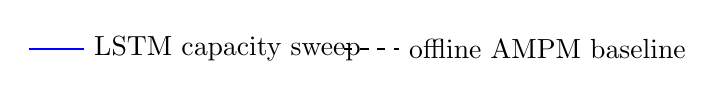
\begin{tikzpicture}[baseline=-0.5ex]
\draw[blue,thick] (0,0)--(0.7,0) node[right,black]{LSTM capacity sweep};
\draw[black,dashed,thick] (4.0,0)--(4.7,0) node[right,black]{offline AMPM baseline};
\end{tikzpicture}
\end{center}

\begin{figure}[H]
\centering
\begin{minipage}{0.49\linewidth}\centering
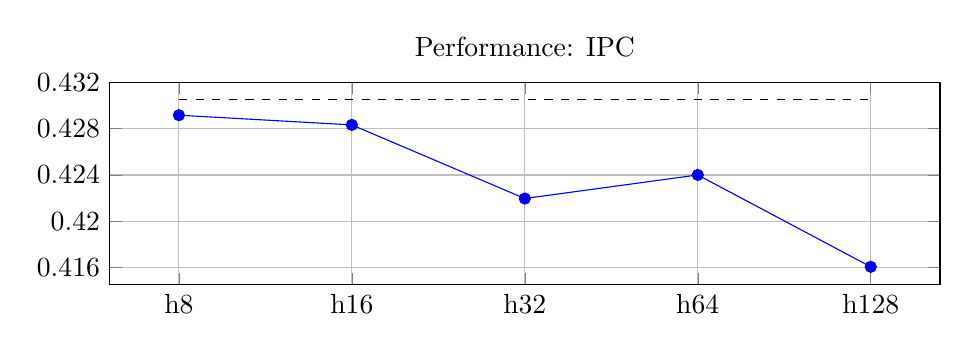
\begin{tikzpicture}\begin{axis}[
width=\linewidth,height=4.15cm,title={Performance: IPC},
xmode=log,log basis x=2,xtick={8,16,32,64,128},xticklabels={h8,h16,h32,h64,h128},
ymin=0.4145,ymax=0.4320,ytick={0.416,0.420,0.424,0.428,0.432},grid=major,
yticklabel style={/pgf/number format/fixed,/pgf/number format/precision=3}]
\addplot[blue,mark=*] coordinates {(8,0.42917)(16,0.42833)(32,0.42196)(64,0.42400)(128,0.41605)};
\addplot[black,dashed] coordinates {(8,0.43054)(128,0.43054)};
\end{axis}\end{tikzpicture}
\end{minipage}
\begin{minipage}{0.49\linewidth}\centering
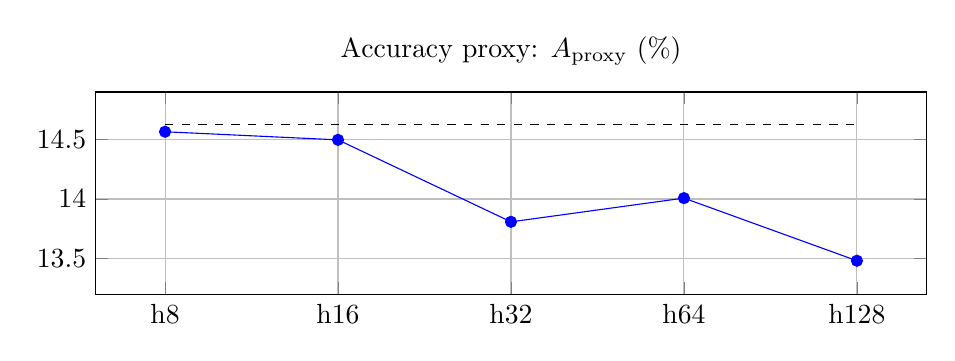
\begin{tikzpicture}\begin{axis}[
width=\linewidth,height=4.15cm,title={Accuracy proxy: $A_{\rm proxy}$ (\%)},
xmode=log,log basis x=2,xtick={8,16,32,64,128},xticklabels={h8,h16,h32,h64,h128},
ymin=13.2,ymax=14.9,grid=major]
\addplot[blue,mark=*] coordinates {(8,14.5654)(16,14.4973)(32,13.8082)(64,14.0077)(128,13.4811)};
\addplot[black,dashed] coordinates {(8,14.6293)(128,14.6293)};
\end{axis}\end{tikzpicture}
\end{minipage}

\begin{minipage}{0.49\linewidth}\centering
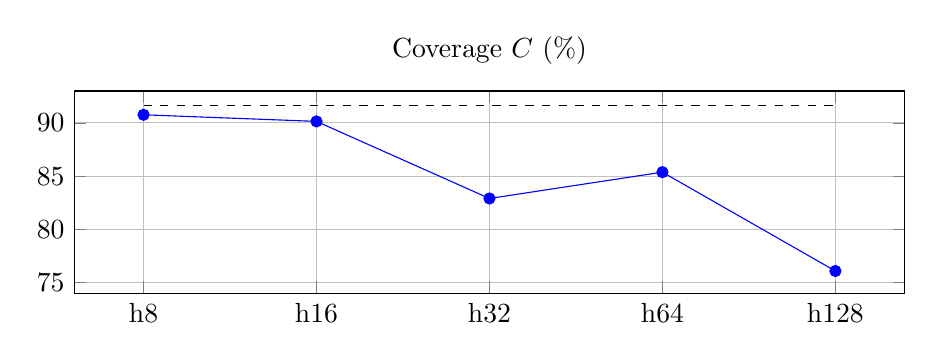
\begin{tikzpicture}\begin{axis}[
width=\linewidth,height=4.15cm,title={Coverage $C$ (\%)},
xmode=log,log basis x=2,xtick={8,16,32,64,128},xticklabels={h8,h16,h32,h64,h128},
ymin=74,ymax=93,grid=major]
\addplot[blue,mark=*] coordinates {(8,90.7606)(16,90.1399)(32,82.8992)(64,85.3705)(128,76.0829)};
\addplot[black,dashed] coordinates {(8,91.6064)(128,91.6064)};
\end{axis}\end{tikzpicture}
\end{minipage}
\begin{minipage}{0.49\linewidth}\centering
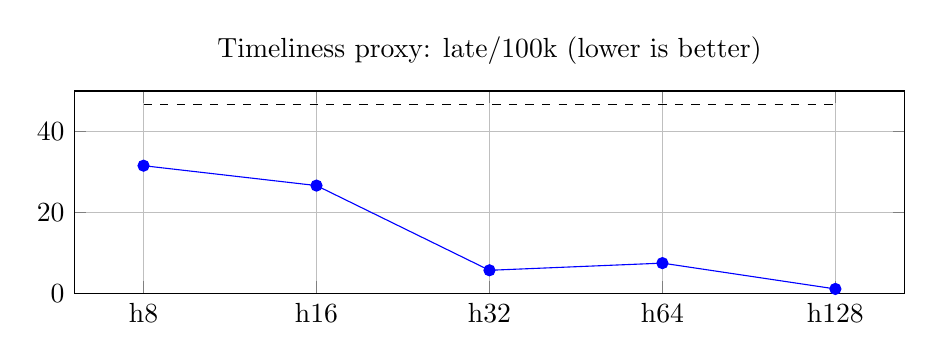
\begin{tikzpicture}\begin{axis}[
width=\linewidth,height=4.15cm,title={Timeliness proxy: late/100k (lower is better)},
xmode=log,log basis x=2,xtick={8,16,32,64,128},xticklabels={h8,h16,h32,h64,h128},
ymin=0,ymax=50,grid=major]
\addplot[blue,mark=*] coordinates {(8,31.5226)(16,26.6032)(32,5.6580)(64,7.4314)(128,1.0468)};
\addplot[black,dashed] coordinates {(8,46.6990)(128,46.6990)};
\end{axis}\end{tikzpicture}
\end{minipage}
\caption{The legend is outside the axes. Lower late density does not compensate for the simultaneous loss of useful-hit yield and coverage.}
\end{figure}

\section*{Data-to-insight map}
\begin{center}\small
\begin{tabularx}{\textwidth}{@{}p{0.22\textwidth}p{0.32\textwidth}X@{}}
\toprule
Question & Data pattern & Supported insight \\
\midrule
Why does h8 miss the baseline? & $U:-1{,}718$, L2 misses:$+1{,}718$, late:$-195$. & Lost useful coverage dominates the timeliness improvement.\\
Does widening approach a crossing? & Every $\Delta$IPC is negative; h128: $-0.01449$. & No saturation crossing is observed; size alone is not the solution.\\
Why can fewer late events still lose? & h128 has only 12 late events but coverage falls to 76.08\%. & Suppressing useful requests makes late density look good while harming performance.\\
\bottomrule
\end{tabularx}
\end{center}

\section*{Conclusion and evidence boundary}
\begin{itemize}
\item \textbf{Result:} no tested matched-input LSTM beats offline AMPM; h8 is closest at $-0.00137$ IPC.
\item \textbf{Mechanism supported by current counters:} the gate removes useful AMPM candidates; coverage loss exceeds timeliness benefit.
\item \textbf{Not yet supported:} strict hardware accuracy, exact lead time, pollution, queue pressure, or cross-seed generalization.
\item \textbf{Next test:} keep AMPM inputs/candidates fixed; train a coverage-preserving utility/ranking objective and calibrate request budget without evaluation-IPC selection.
\end{itemize}

\section*{Verified provenance}
Analyzer status \texttt{PASS}; canonical content SHA256 prefixes: \texttt{2564c753145a} (train), \texttt{729c2c44e2e6} (guard), and \texttt{36ce707c2f27} (evaluation). Live AMPM is a validated reference (0.43069 IPC), not the primary offline comparator.

\end{document}
